
\documentclass[a4paper,11pt,oneside]{memoir}

% Style of front page, title page, and stuff page
\usepackage{dikuReport}

%% Packages
% Formatting
\usepackage[utf8]{inputenc}
\usepackage{latexsym}
\usepackage[T1]{fontenc}
\usepackage{relsize}
\usepackage{fix-cm}
\usepackage{cite}
\usepackage{tikz}
\usepackage{graphicx}
\usepackage{color}
\usepackage{amsbsy}
\usepackage{amssymb}
\usepackage{amsmath}
\usepackage{float}
\usepackage{xspace}
\usepackage{listings}
\usepackage{url}
\usepackage{booktabs}
\usepackage{nameref}

\usepackage{array}
\usepackage{makecell}

\usepackage[colorinlistoftodos,prependcaption,textsize=tiny]{todonotes}


\DeclareUnicodeCharacter{00A0}{~}
\usetikzlibrary{arrows, automata}

%%%%% Make abbreviations emphasized. Use if you like.
\newcommand{\ie}{\emph{i.e.}\xspace}
\newcommand{\eg}{\emph{e.g.}\xspace}
\newcommand{\etc}{\emph{etc.}\xspace}
\newcommand{\vs}{\emph{vs.}\xspace}
\newcommand{\cf}{\emph{cf.}\xspace}
\newcommand{\viz}{\emph{viz.}\xspace}
\newcommand{\etal}{\emph{et~al.}\xspace}

\newcommand{\tbf}[1]{\textbf{#1}}
\newcommand{\tit}[1]{\textit{#1}}
\newcommand{\ttt}[1]{\texttt{#1}}

\renewcommand\theadalign{bc}
\renewcommand\theadfont{\bfseries}
\renewcommand\theadgape{\Gape[4pt]}
\renewcommand\cellgape{\Gape[4pt]}

%http://detexify.kirelabs.org/classify.html

%Auto label sections either by [sub[sub]]section/chapter[label]{name}, or just [sub[sub]]section/chapter{label=name}
% Chapters
\let\orichaptermark\chaptermark
\renewcommand\chaptermark[1]{\label{chp:#1}\orichaptermark{chp:#1}}
% Sections
\let\orisectionmark\sectionmark
\renewcommand\sectionmark[1]{\label{sec:#1}\orisectionmark{sec:#1}}
% Subsections
\let\orisubsectionmark\subsectionmark
\renewcommand\subsectionmark[1]{\label{ssec:#1}\orisubsectionmark{ssec:#1}}
% Subsubsections
\let\orisubsubsectionmark\subsubsectionmark
\renewcommand\subsubsectionmark[1]{\label{sssec:#1}\orisubsubsectionmark{sssec:#1}}

% Where graphic files are located
\graphicspath{{figures/}}

\begin{document}

%%%%%%%%%%%%%%%%%%%%%%%%%%%%%%%%
% Basic information
%%%%%%%%%%%%%%%%%%%%%%%%%%%%%%%%
\thesistype{MSc thesis}

\thesiscomment{} % You can leave this blank
\title{Using Model-Based testing to test MCP Instance-Specifications}
\subtitle{Rage Against the Finite State Machine: Boats on Parade} % If you want one; if not '~'
\author{Søren Lund Hess-Petersen - pws412}
\supervisor{Michael Kirkedal Thomsen\\<m.kirkedal@di.ku.dk>}
\date{\today} % Hand-in date

\pagestyle{plain}
\maketitle

\cleardoublepage
\pagenumbering{roman}
\setcounter{page}{3}

\cleardoublepage
\pagestyle{plain}

% English Abstract
\begin{abstract}
\TODO{Write when done} 
\end{abstract}

% Danish abstract
\begin{resume}
\TODO{Write when done} 
\end{resume}

\chapter*{Preface}
This Master's thesis is submitted in fulfilment of the master programme in Computer Science at the University of Copenhagen for Søren Lund Hess-Petersen.


\cleardoublepage
\chapterstyle{combined}
\tableofcontents*

% Starting the real text.
\cleardoublepage
\pagenumbering{arabic}
\setcounter{page}{1}


% It can be an advantage to seperate some of the following chapters into seperate files.
% Make a bachground.tex and include with \input{background}

%%%%%%%%%%%%%%%%%%%%%%%%%%%%%%%%%%%%%%%%%%%%%%%%%%%%%%%%%%%%%%%%%%%%%%%%%%%%%%%
%%% Introduction                                                            %%%
%%%%%%%%%%%%%%%%%%%%%%%%%%%%%%%%%%%%%%%%%%%%%%%%%%%%%%%%%%%%%%%%%%%%%%%%%%%%%%%

\chapter{Introduction}
The Maritime Connectivity Platform \cite{mcp} (MCP) is, as the name suggests a platform that connects maritime services, functioning as a common infrastructure by offering safe and reliable information exchange between various maritime actors. A particular way of utilizing this is that a user of the MCP is able to develop his or her own software, and distribute it across the world. Such digital maritime components, however needs to be thoroughly tested, which often is not adequately done through simple unit testing. Thus, software components, distributed through the MCP need a thorough test-suite, for which the obvious solution is to implement model-based testing.
The MCP has provided specifications, which describe rules that software needs to adhere to. These specifications will be used to create the model, that will verify the software. The specifications are provided in \ttt{xml}-format, and are, as of now, not used in any formal degree. Ideally, the provided specifications should be used to automatically generate models, which can be used to verify that a certain piece of software adheres to the specification. 
\section{Description of the Project}
In this project, QuickCheck \cite{quickcheck} will be utilized in order to verify that instances fulfills the requirements set by specifications in the MCP.
QuickCheck is a library, which allows for model-based testing of software. Originally, QuickCheck was written in Haskell, but has since been extended to more than 50 programming languages. The idea behind this method is, as the term \tit{model}-based testing suggests, to create models which describe the properties that the test-cases need to reflect. This means that in stead of conducting unit-tests, the model should reflect what needs to happen with an arbitrary input- and function-combination, and ideally catch every special case that either has not been accounted for in the model or in the analysed software.
Once an accurate model is created further testing can be streamlined, as a simple test can affirm an entire aspect of the tested software, in stead of just \tit{one} particular example.
The goal of the project is to create an automatic test suite for the MCP, which performs better than a unit-based test suite. In the long run, such a test suite has the capacity to increase reliability, efficiency and ultimately make way for better distributed, and more uniformly created software components in the Maritime Connectivity Platform. 
\section{Learning Objectives}

\begin{itemize}
	\item Utilizing QuickCheck in creating viable models, that describe the specifications, provided in MCP specifications.
	\item Interpreting MCP specifications in order to generate relevant tests.
	\item Parsing MCP specifications in order to generate relevant models.
	\item Applying property-based testing of functions and specifications in a maritime environment.
\end{itemize}

\section{Scope}

\section{Limitations}

\section{Structure}

\begin{itemize}
	\item \tbf{Chapter \refNumName{chp:Background}}\\
	This chapter describes the techniques, theories, and components that are used or analyzed throughout the thesis.
	\item \tbf{Chapter \refNumName{chp:Analysis}}%\\
	%TODO Description of Chapter 3
	\item \tbf{Chapter \refNumName{chp:Work/Design}}%\\
	%TODO Description of Chapter 4
	\item \tbf{Chapter \refNumName{chp:Results}}%\\
	%TODO Description of Chapter 5
	\item \tbf{Chapter \refNumName{chp:Discussion}}%\\
	%TODO Description of Chapter 6
	\item \tbf{Chapter \refNumName{chp:Conclusion}}%\\
	%TODO Description of Chapter 7
\end{itemize}
\displayCounterChp

%%%%%%%%%%%%%%%%%%%%%%%%%%%%%%%%%%%%%%%%%%%%%%%%%%%%%%%%%%%%%%%%%%%%%%%%%%%%%%%
%%% Background                                                              %%%
%%%%%%%%%%%%%%%%%%%%%%%%%%%%%%%%%%%%%%%%%%%%%%%%%%%%%%%%%%%%%%%%%%%%%%%%%%%%%%%

\chapter{Background}

\section{The Maritime Connectivity Platform}
The Maritime Connectivity Platform (MCP), formally known as the Maritime Cloud, is a platform, developed by EfficienSea2~\cite{efficienSea2}, which is led by the Danish Maritime Authority. 
MCP is a communication framework, that is to ensure efficient, reliable and secure communication, and exchange of information in the maritime sector.
The goal of the platform is to connect maritime stakeholders with maritime information services.
\begin{figure}
  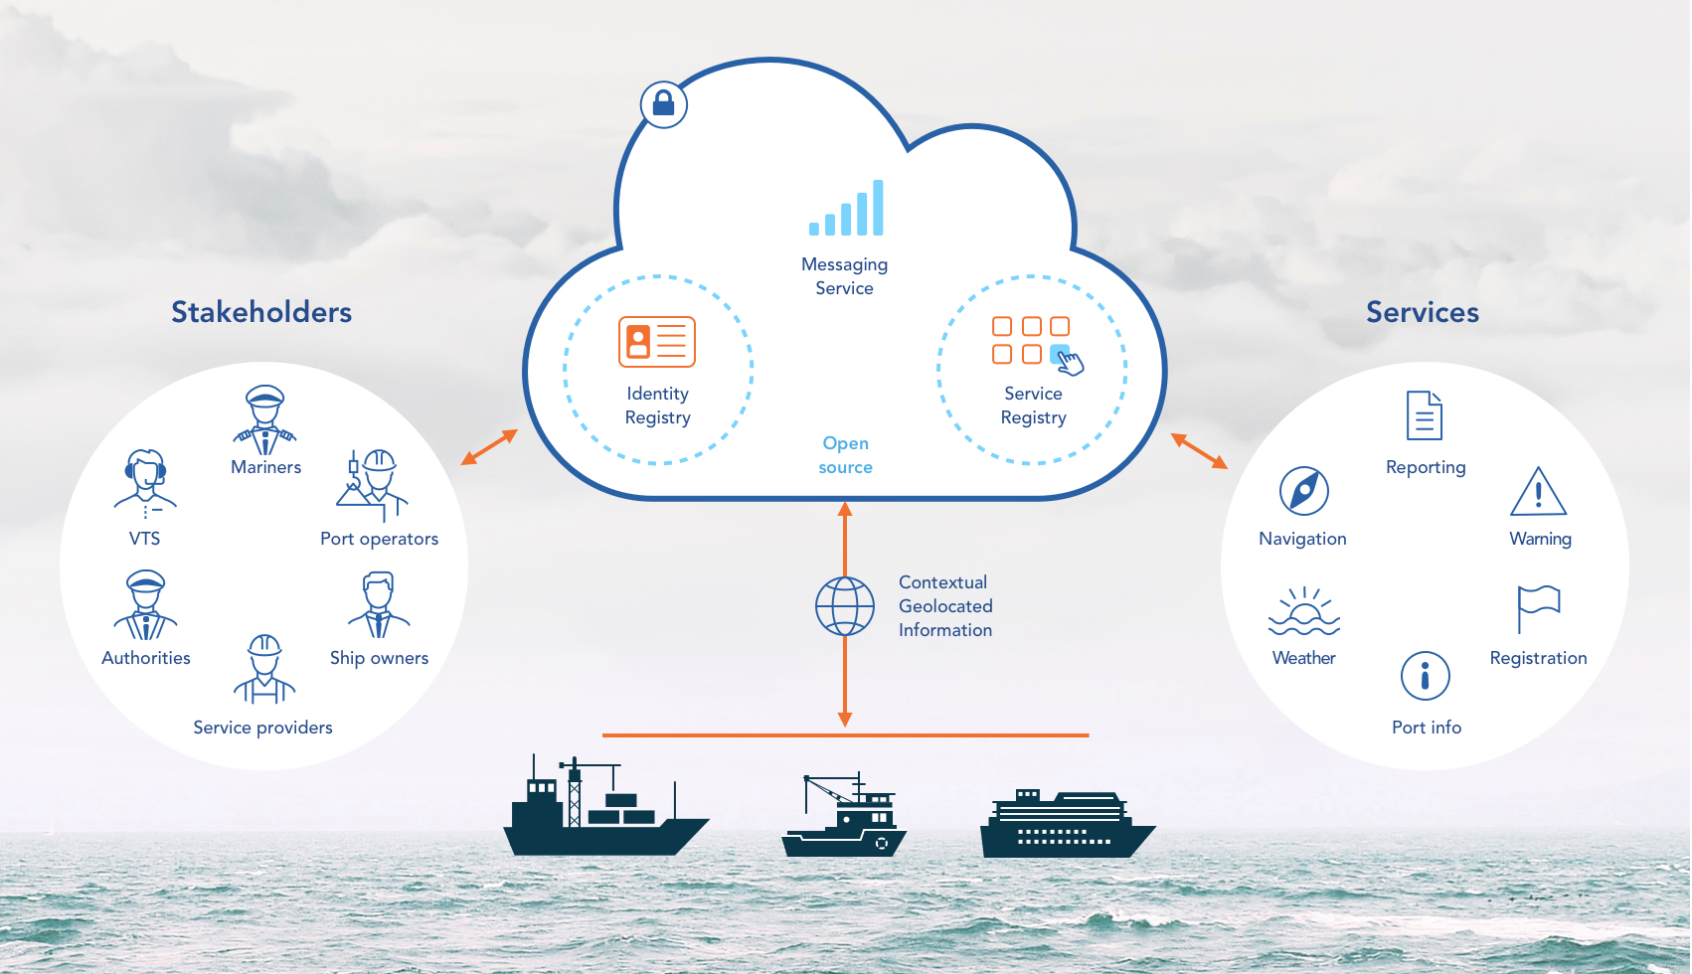
\includegraphics[width=1\textwidth]{figures/MCPStructure}
  \caption{Diagram, describing the structure of MCP~\cite{efficienSea2}.}
  \label{fig:MCPStruct}
\end{figure}\noindent
A high-level diagram, describing the structure of the MCP can be seen in Figure~\ref{fig:MCPStruct}. Here it is shown that maritime stakeholders are connected with the maritime services through the Identity Registry, the Service Registry and the Messaging Service.

\subsection{Identity Registry}
Here the relevant information regarding maritime stakeholders are stored. This information needs to be authorized and stored at a safe location in order for the security of the MCP to be sufficient. The Identity Registry on the MCP is equivalent to the Central Person Registry of a country. The Identity Registry is vital to the MCP, in that it ensures the solution's authenticity, integrity, and confidentiality. Maritime stakeholders are, through the Identity Registry, provided with a single login to all Maritime Services~\cite{efficienSea2}.
\subsection{Service Registry}
What the Identity Registry provides for the Maritime Stakeholders, the Service Registry provides for the Maritime Services. Here all Maritime Services are registered and stored. The Service Registry provides both commercial and non-commercial, as well as authorized and non-authorized services, either free of charge or for a fee. The Service Registry is comparable with the App Store or Google Play, in that it distributes services of all kinds to registered users~\cite{efficienSea2}.
\subsection{Messaging Service}
The messaging service in the MCP, enables the exchange of information across the different platforms, thereby linking their systems to each other. The messaging service accounts for the available means of communication, as well as the geographical coordinates of the destination and origin of the information, being sent~\cite{efficienSea2}.

\section{Parsing}
Parsing is a widely known tool in computer science. The term expresses a function, taking a string of input, from which it yields a parse tree that it constructs when applying the specific parser logic upon the input string. The parser performs a lexical analysis, meaning that it converts sections of the string to tokens, that are ultimately easier to handle by an interpreter. When using Erlang to define parsers, a library family known as parser combinators is very popular, in that it allows the programmer to embed domain specific language directly into the parser. The concept of combinatory parsing is using one or more of these libraries of higher-order functions, known as parser combinators. Parser combinators take in parsers of any kind imaginable as input and returns a new set of parsers as an output.
\newpage
\subsection{Monadic Parsing}
Before 1995, implementation of top-down parsing, using parser combinators ran in and used both exponential time and space complexity, when applied to ambiguous, context free grammars. At that time Frost and Szydlowski demonstrated that memoization can enhance parser combinators in order to optimize time complexity to polynomial~\cite{memoization}. One year later through the use of monads, Haskell-specific parser combinators were reconstructed by Frost which introduced systematic and correct threading of memoization throughout execution.

\section{Interpretation}
In solutions, utilizing parsers, an interpreter is often introduced to handle the result that the parser returns, and for this reason, interpreters share the same syntax that is used in their corresponding parsers. The job of an interpreter is to execute the parsed commands, and therefor their implementation can vary to an even higher extend than that of a parser. Often-times a parser-interpreter combination is used to identify, generate, as well as execute domain-specific languages. Since automatic utilization of domain-specific language is an integral part of the problem-statement, using a parser- and interpreter-combination is straightforward to the solution.

\section{Property-Based Testing}

Property-based testing, also known as Automation Testing, is the principle of testing properties of code, rather than instances, as is done in manual unit testing. Unit tests are fast and easy to set up and execute, however, in most instances they only provide coverage to a certain degree.

\begin{figure}[h]
  \centering
  \begin{lstlisting}
import Test.QuickCheck
import Data.List

qsort :: Ord a => [a] -> [a]
qsort []     = []
qsort (x:xs) = qsort lhs ++ [x] ++ qsort rhs
    where lhs = filter  (< x) xs
          rhs = filter (>= x) xs

prop_idempotent xs = qsort (qsort xs) == qsort xs
  \end{lstlisting}
  \caption{Example of Property-Based Testing~\cite{realWorldHaskell11}}.
  \label{fig:pbtEx}
\end{figure}\ \\

\noindent
Depending on the complexity of the given program, most programmers can come up with tests, covering most of the given program, however, many edge-cases are unintuitive and would require extensive testing to discover manually. Property-based testing solves this problem by setting up test cases that take into account mathematical models, describing the desired behavior of the code. Once such a test case has been created, semi-random execution instances can be run to the point of literal exhaustion, and thus a relatively small program can test for thousands of occurrences at once.

An example of this can be seen in Listing~\ref{fig:pbtEx}, which describes a snippet of Haskell quicksort code. A property of quicksort is that a list, sorted once is equivalent to that list, sorted twice, and this is what the function \lstinline{prop_idempotent} validates.

\section{Model-Based Testing}

The principle of Model-based testing is to check behavior of software against predictions made by a model. Behavior can be described in a variety of manners, including data flow, control flow, dependencies, decision trees/cycles, and state transition machines. Model-based testing is good at describing the behavior of a system, when it reacts to a specific action, which is determined by another specific model. Using this technique, the behavior of a system can easily be determined and validated. Currently there are two main types of model-based testing-techniques:

\begin{description}
  \item[Serial model building- and testing],
  is a way of implementing model-based testing and involves predefined models, upon which a number of tests are executed. Creating the tests manually ahead of execution allows the tester to implement an additional layer of complexity to the created models. Furthermore, implementing this strain of model-based testing allows for custom-tailored testing, suited to fit issues, unique to the corresponding model. Depending on the amount of models, this is, however, a significantly slower process than the alternative, in that each model requires a similar amount of time to construct. Depending on the developer, as well as the implementation techniques of models, a relatively high leaning curve may be introduced, leading to exclusions of parties, not qualified to take on this task. 
  Figure~\ref{fig:serialMBT} provides a high-level diagram, describing this principle, using arbitrary measurement units of time consumption, skill level, and model complexity along its $y$-axis, and amount of models along its $x$-axis. \newpage
  \begin{figure}[h]
    \centering
    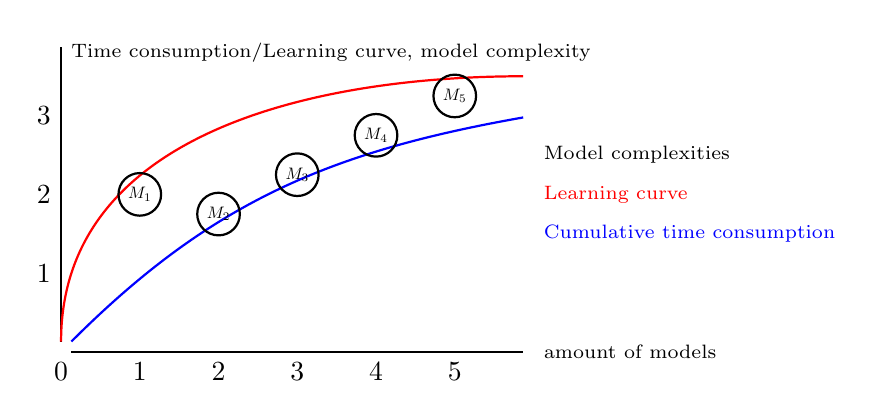
\begin{tikzpicture}[thick]
      % horizontal and vertival axis
      \node (Z) at (0,0) {};
      \node (X) at (6,0) {};
      \node (Y) at (0,4) {};

      \path [] (Z) edge (X);
      \path [] (Z) edge (Y);

      % horizontal labels
      \draw (0,0) node[anchor=north]  {0}
            (1,0) node[anchor=north]  {1}
            (2,0) node[anchor=north]  {2}
            (3,0) node[anchor=north]  {3}
            (4,0) node[anchor=north]  {4}
            (5,0) node[anchor=north]  {5}

      % vertical labels
            (0,1) node[anchor=east] {1}
            (0,2) node[anchor=east] {2}
            (0,3) node[anchor=east] {3};
      
      \node (L) at (6,3.5) {};
      \node (T) at (6,3) {};

      \path [red, out=90, in=180] (Z) edge (L);
      \path [blue,out=45, in=190] (Z) edge (T);

      \draw (6,2.5) node[anchor=west] {\scriptsize\color{black} Model complexities}
            (6,2)   node[anchor=west] {\scriptsize\color{red}   Learning curve}
            (6,1.5) node[anchor=west] {\scriptsize\color{blue}  Cumulative time consumption};
      
      \draw (0,3.8) node[anchor=west] {\scriptsize Time consumption/Learning curve, model complexity};
      \draw (X)     node[anchor=west] {\scriptsize amount of models};

      \node (M1)  [circle,  draw, scale=0.6] at (1,2)   {$M_1$};
      \node (M2)  [circle,  draw, scale=0.6] at (2,1.75)  {$M_2$};
      \node (M3)  [circle,  draw, scale=0.6] at (3,2.25)  {$M_3$};
      \node (M4)  [circle,  draw, scale=0.6] at (4,2.75)  {$M_4$};
      \node (M5)  [circle,  draw, scale=0.6] at (5,3.25)  {$M_5$};
    \end{tikzpicture}
    \caption{Time consumption and learning curve of serial model building and testing.}
    \label{fig:serialMBT}
  \end{figure}\ \\
  Figure~\ref{fig:serialMBT} shows the time consumption increasing for every model built, while the learning curve initiates very steeply, however diverges, as the creator of the models learns the used techniques. 
  \item[Sequential model building- and testing],
  is a way of implementing model-based testing, that involves on-the-fly model creation- and testing. Here, a program is designed to take in arguments, describing different model behaviors, upon the basis of which the program tests the models immediately after they are generated. Compared with the implementation described above, this technique scales to a much better degree, as the program will only need to be written once in order to create a virtually infinite amount of models. 
  Input, containing all necessary information that would otherwise be entered manually is, however, still needed, and thus scalability is not completely eliminated. 

  Figure~\ref{fig:sequenceMBT} provides a high-level diagram, describing this principle, using arbitrary measurement units of time consumption, skill level, and model complexity along its $y$-axis, and amount of models along its $x$-axis.
  \begin{figure}[h]
    \centering
    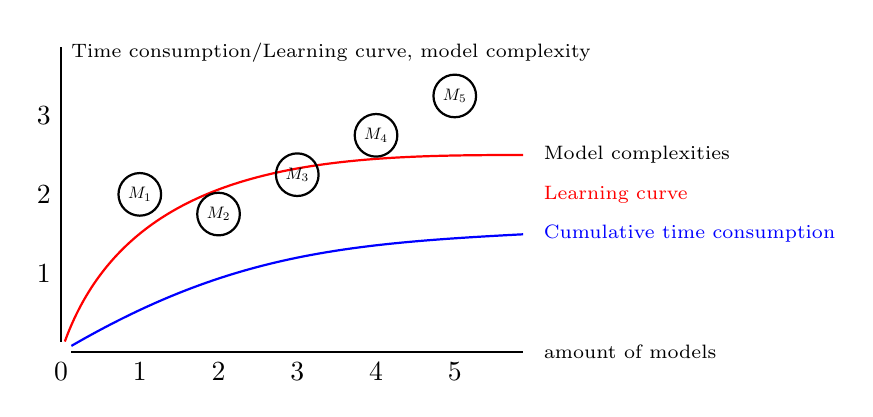
\begin{tikzpicture}[thick]
      % horizontal and vertival axis
      \node (Z) at (0,0) {};
      \node (X) at (6,0) {};
      \node (Y) at (0,4) {};

      \path [] (Z) edge (X);
      \path [] (Z) edge (Y);

      % horizontal labels
      \draw (0,0) node[anchor=north]  {0}
          (1,0) node[anchor=north]  {1}
          (2,0) node[anchor=north]  {2}
          (3,0) node[anchor=north]  {3}
          (4,0) node[anchor=north]  {4}
          (5,0) node[anchor=north]  {5}

      % vertical labels
          (0,1) node[anchor=east] {1}
          (0,2) node[anchor=east] {2}
          (0,3) node[anchor=east] {3};
      
      \node (L) at (6,2.5){};
      \node (T) at (6,1.5){};

      \path [red, out=70, in=180] (Z) edge (L);
      \path [blue,out=30, in=183] (Z) edge (T);

      \draw (6,2.5) node[anchor=west] {\scriptsize\color{black} Model complexities}
          (6,2) node[anchor=west] {\scriptsize\color{red}   Learning curve}
          (6,1.5) node[anchor=west] {\scriptsize\color{blue}  Cumulative time consumption};
      
      \draw (0,3.8) node[anchor=west] {\scriptsize Time consumption/Learning curve, model complexity};
      \draw (X)     node[anchor=west] {\scriptsize amount of models};

      \node (M1)  [circle,  draw, scale=0.6] at (1,2)   {$M_1$};
      \node (M2)  [circle,  draw, scale=0.6] at (2,1.75)  {$M_2$};
      \node (M3)  [circle,  draw, scale=0.6] at (3,2.25)  {$M_3$};
      \node (M4)  [circle,  draw, scale=0.6] at (4,2.75)  {$M_4$};
      \node (M5)  [circle,  draw, scale=0.6] at (5,3.25)  {$M_5$};
    \end{tikzpicture}
    \caption{Time consumption and learning curve of sequential model building and testing.}
    \label{fig:sequenceMBT}
  \end{figure}\\
  Like Figure~\ref{fig:serialMBT}, Figure~\ref{fig:sequenceMBT} introduces a learning curve, as the user will need to become familiar with the input needing to be specified, in order for the sequential model creation to start, however, this is severely more gradual, while also featuring a lower end-point than the one seen in Figure~\ref{fig:serialMBT}. The cumulative time consumption is also lower, compared to serial model building, due to the fact that this process will run semi-automatically, only needing input from a user, before handling all building-related tasks.
\end{description}
\newpage
\subsection{Finite State Machines (FSM)}
A finite state machine is, as the name suggests, a mathematical machine, consisting of a collection of states and actions. An arbitrary FSM has a start state along with a collection of states that are accessed through various status- and/or input-combinations. An example of this can be seen in Figure~\ref{fig:fsmEx}, which describes the flow of a turnstile, which allows for one pass through, after which it prompts for a coin before allowing another pass through.

\begin{figure}[h]
  \centering
  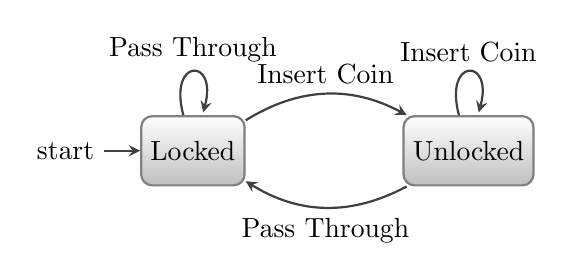
\begin{tikzpicture}[->,>=stealth', node distance=3.5 cm, thick]
    \tikzstyle{every state}=[rectangle,
                       draw=gray,
                       rounded corners,
                       rectangle,
                       top color=white,
                       bottom color=gray!50]
    \tikzstyle{every path}=[->,gray!150,>=stealth,text=black]

    \node[state, initial] (A) []      {Locked};
    \node[state]      (B) [right of=A]{Unlocked};

    \path (A) edge  [bend left, above]  node  {Insert Coin} (B)
          edge  [loop above,above]  node  {Pass Through}  (A)
        (B) edge  [loop above,above]  node  {Insert Coin} (B)
          edge  [bend left, below]  node  {Pass Through}  (A);
  \end{tikzpicture}
  \caption{Example of a finite state machine, describing a turnstile. Furthermore, this figure describes Table~\ref{tab:fsmEx}.}
  \label{fig:fsmEx}
\end{figure}
In addition to describing the concept of states in a FSM, Figure~\ref{fig:fsmEx} and Table~\ref{tab:fsmEx} also displays a collection of actions. An action is an operation that is performed along with a corresponding state, which can potentially change that state. The described case, features the two actions 'Insert Coin' and 'Pass Through'. The action 'Insert Coin' alters the state of the turnstile, only if performed when the state of the turnstile is 'Locked', as it is not possible to unlock an already unlocked lock. Similarly, the action 'Pass Through' only changes the state if the turnstile is in its unlocked state before performing the action, as passing through a locked turnstile is not possible.
\newpage
\noindent
Table~\ref{tab:fsmEx}, seen below displays the relationships between the actions, states and output, produced when interacting with the turnstile, using its intended functionality. The table features the four columns, with 'State' describing the state before execution of the 'Action' column. 'Next State' describes the state after the action has taken effect, and the 'Output' column describes the flow of events, leading to the next state. Note that the Output column features event flows that do \tit{not} lead to a change in state, as well as outcomes that do.
\begin{table}[h]
  \centering
  \begin{tabular}{l|l|l|l}\toprule
    State   & Action    & Next State& Output \\ \midrule
    Locked    & Insert Coin & Unlocked  & \colorbox{green}{Unlocks turnstile, allowing passage.} \\
    Locked    & Push      & Locked  & \colorbox{red}{Blocks passage.} \\
    Unlocked  & Insert Coin & Unlocked  & \colorbox{green}{Returns coin.} \\
    Unlocked  & Push      & Locked  & \colorbox{red}{Allows passage, locks.} \\ \bottomrule
  \end{tabular}
  \caption{Example of a finite state machine, describing a turnstile. Furthermore, this table describes Figure~\ref{fig:fsmEx}.}
  \label{tab:fsmEx}
\end{table}
\displayCounterChp

%%%%%%%%%%%%%%%%%%%%%%%%%%%%%%%%%%%%%%%%%%%%%%%%%%%%%%%%%%%%%%%%%%%%%%%%%%%%%%%
%%% Analysis                                                                %%%
%%%%%%%%%%%%%%%%%%%%%%%%%%%%%%%%%%%%%%%%%%%%%%%%%%%%%%%%%%%%%%%%%%%%%%%%%%%%%%%

\chapter{Analysis}

In this chapter, I will present and analyze the data made available by the MCP in the three documents \ttt{E2 - NW-NM DMA Service Instance}, \ttt{E2 - NW-NM REST Service Technical Design}, and \ttt{E2 - NW-NM Service Specification}, which represent all data, made available to me. Furthermore, I will explain the necessity of testing the MCP, as well as present a description of a favorable model structure and potential methods of generating said models.

\section{Data}

To provide a holistic description of a service instance, three documents are necessarily provided. Below are the descriptions of the documents with the service instance \ttt{E2 - NW-NM DMA} as an example.
\begin{description}
  \item[E2 - NW-NM DMA Service Instance]\ \\
    The purpose of this service instance document and its xml-defined counterpart is to describe a DMA instance of the REST-based technical design of the MW- NM service specification, according to the guidelines given in the Service Description Guidelines.
  \item[E2 - NW-NM REST Service Technical Design]\ \\
    The purpose of this service technical design document and its xml-defined counterpart is to describe a REST-based technical design of the MW-NM service specification, according to the guidelines given in the Service Description Guidelines.
  \item[E2 - NW-NM Service Specification]\ \\
    The purpose of this service specification document and its xml-defined counterpart is to provide a holistic overview of the MW-NM service and its building blocks in a technology-independent way, according to the guidelines given in the Service Description Guidelines.
\end{description}
Of the three documents, only the last, \ttt{Service Specification} is to be used to describe specifications of the service, and as such only this will be studied closer.
\section{Service Specification grammar}
The service specification document is constructed using a general xml-format. The majority of the parser grammar of the document can be seen in Figure~\ref{fig:sSpecFull} as well as in Figure~\ref{fig:sSpecRed}, while the latter is in a severely reduced and generalized form. A minority of the grammar has been cut from Figure~\ref{fig:sSpecFull} as it was deemed irrelevant, however the parser grammar in its entirety can be seen in appendices,~\ref{fig:sSpecFull1} and~\ref{fig:sSpecFull2}.

\begin{figure}
  \centering
  \begin{lstlisting}[keywordstyle={}]
ServiceSpecificationSchema ::= specifications

specifications ::= spec specifications
    | $\e$
     
spec ::= name
    | status
    | ID
    | version
    | description
    | keywords
    | isSpatialExclusive
    | authorInfos
    | requirements
    | serviceDataModel
    | serviceInterfaces
     
authorInfos ::= authorInfo authorInfos
    | $\e$

authorInfo ::= aSpec authorInfo
    | $\e$

aSpec ::= ID
    | name
    | description
    | contactInfo

requirements ::= requirement requirements
    | $\e$

requirement ::= rSpec requirement
    | $\e$

rSpec ::= ID
    | name
    | text

serviceDataModel ::= definitionAsXSD

serviceInterfaces ::= serviceInterface serviceInterfaces
    | $\e$

oSpec ::= name
    | description
    | returnValueType
    | parameterTypes
  \end{lstlisting}
  \caption{Snippets of full parser grammar of Service Specification Schema. (Found in appendices~\ref{fig:sSpecFull1}, and~\ref{fig:sSpecFull2})}
  \label{fig:sSpecFull}
\end{figure}

\begin{figure}
  \centering
  \begin{lstlisting}[keywordstyle={}]
ServiceSpecificationSchema ::= specifications

specifications ::= spec specifications
    | $\e$
     
spec ::= specifications
    | spec
    | $\e$

spec ::= string
  \end{lstlisting}
  \caption{Reduced parser grammar of Service Specification Schema.}
  \label{fig:sSpecRed}
\end{figure}

As mentioned above, the service specification is to be used to verify the behavior of the maritime service from a technical stand point. At the moment, the xml-document provides a technical description of its corresponding maritime service, but the most commonly used expression method is free text. As this is a very non-technical design choice, a large portion of the obvious technical advantages provided by the xml-format, is lost. 

As it is possible to utilize free text though the use of natural language processing~\cite{nlp}, no modifications are strictly necessary, however, even with utilization of such or similar methods, implementation hereof would be unstable in terms of usability. This is due to the fact that free language formulation varies at an unforeseeable degree, and as such creating uniform models based on this would add a great layer of complexity.

For a more sustainable solution to the problem, see Section~\ref{sec:Updated Data}.

The xml-version of the service specification can be found in Appendix~\ref{sec:E2 - NW-NM Service Specification}.

\section{Testing the MCP}

The core principle in the MCP is to restructure and streamline maritime software sharing in a manner that can be done the world over, and the very nature of this statement dictates that the platform must be highly scalable. This adds the necessity of running quality-checks on all of the maritime services that are uploaded to the platform. To accommodate this issue, model-based testing immediately seems like the obvious solution, as this technique covers most of the required desired functionality. If implemented satisfyingly, a model-based testing suite for the MCP would be able to:
\begin{enumerate}
  \item Present or verify behavior of maritime services.\\
    There are many obvious common behavioral traits of maritime services, such as adding ships and maritime stakeholders, as well as removing them, however other behavioral patterns will often vary to the point of lowered manageability. A model, describing the maritime service in question will provide a clear and undeniable description of the service's behavior.\newpage
  \item Visualize functionality of maritime services.\\
    Just as well as behavioral traits, functionality will differ greatly from one maritime service to another, and therefore it is very useful for a model to visualize said functionality, as well as verifying that it works as intended.
  \item Present the structures of maritime services.\\
    This trait will be used to visualize the structural components of maritime services. Just as point one and two, this functionality will be useful for creating a quick and clear projection of how the maritime service behaves.
  \item Increase reliability and efficiency of maritime services.\\
    Through correct implementation of points one, two, and three, it is possible to elevate the reliability and efficiency of the maritime services, found on the MCP. This is due to the same reasoning that all testing is conducted on the basis of: the need for safe, consistent, and correct code.
\end{enumerate}
\noindent
As stated in Section~\ref{sec:Model-Based Testing} there are two main types of model-based testing techniques: serial and sequential model building-and testing, and as these two techniques both provide different advantages utilizing either one will be a trade-off.\newpage

\section{Example Model Structure}
Throughout this report, I will use a map-requesting service as an example. In this example the maritime service will act as an intermediate, broking between a ship and a company, where the map is being held. The ship will have to submit authentication information to the maritime service in order to get a the requested map. The model, which has been built upon the example protocol has been illustrated in Figure~\ref{fig:modelExProtocol}. The lines numbered 1-6 illustrate interaction between the three entities \ttt{Ship}, \ttt{Service}, and \ttt{Company}, where *1 and *2 respectively, illustrate a submitting of authentication information to the service, and the service accepts the information and sends a response. *3 and *4 illustrates the service's request of the requested map, and its subsequent receiving hereof. *5 illustrates the forwarding of requested information to the ship.
\begin{figure}[h!]
  \centering
  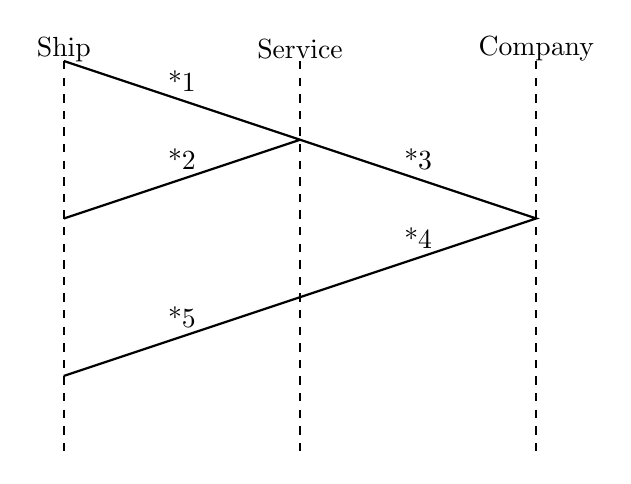
\begin{tikzpicture}[thick]
    % timelines
    \draw [dashed]  (0,5) --  (0,0)
        [dashed]  (3,5) --  (3,0)
        [dashed]  (6,5) --  (6,0);
    % entity labels
    \draw (0,5.15)  node  {Ship}
        (3,5.15)  node  {Service}
        (6,5.15)  node  {Company};

    % interaction labels
    \draw (1.5,4.75)  node  {*1}
        (1.5,3.75)  node  {*2}
        (4.5,3.75)  node  {*3}
        (4.5,2.75)  node  {*4}
        (1.5,1.75)  node  {*5};
    % interaction lines
    \draw (0,5) --  (3,4) --  (0,3) % API call (request/response)
        (3,4) --  (6,3) --  (0,1);  % Service requests/recieves data from company/data center and Information is forwarded to the ship.
  \end{tikzpicture}
  \caption{Early draft of a model example, where a ship requests information from a service.}
  \label{fig:modelExProtocol}
\end{figure}
Figure~\ref{fig:fsmExShip} represents an FSM, illustrating the \ttt{ship} entity in Figure~\ref{fig:modelExProtocol}. The FSM starts in the \ttt{No map loaded} state, and has the three available actions, \ttt{trash map}, \ttt{request map}, and \ttt{await response}. Performing \ttt{trash map} or \ttt{await response} in the initial state will yield no results, as no map is available to be trashed and no response is on the way. If \ttt{request map} is performed, the state will be changed to the intermediate state \ttt{awaiting map}, where \ttt{await response} is the only action that will change the state, as no map can be trashed, and requesting another map will change the state to the same, but where a different map is being waited for. The third and final state \ttt{map loaded} will allow the actions \ttt{trash map}, which will change the state to \ttt{no map loaded} and \ttt{request map}, which will, respectively, trash the loaded map, and request a new one, changing the state to \ttt{awaiting map}.
\newpage
\noindent
Figure~\ref{fig:fsmExService} represents an FSM, illustrating the \ttt{service} entity in Figure~\ref{fig:modelExProtocol}. The FSM has the two states, \ttt{idle} and \ttt{active}, the former being the initial state. Whenever the entity receives a valid response the state changes to the \ttt{active} state, and when the request has been properly handled, the state changes back to \ttt{idle}.
\begin{figure}[h]
  \centering
  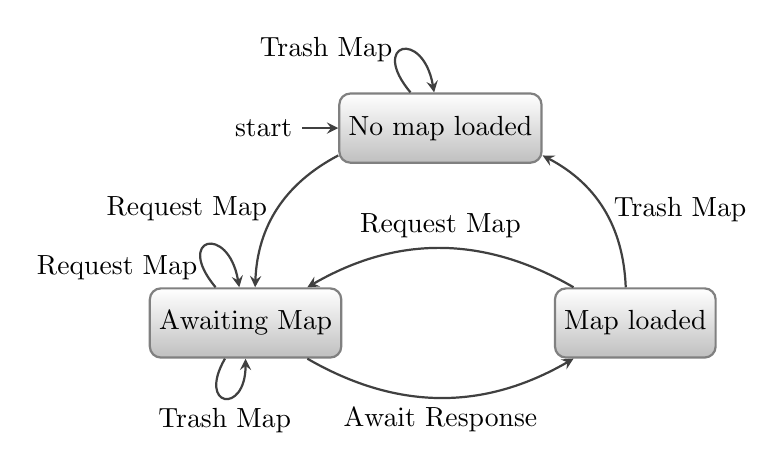
\begin{tikzpicture}[->,>=stealth', node distance=3.5 cm, thick]
    \tikzstyle{every state}=[rectangle,
                       draw=gray,
                       rounded corners,
                       rectangle,
                       top color=white,
                       bottom color=gray!50]
    \tikzstyle{every path}=[->,gray!150,>=stealth,text=black]

    \node[state, initial] (A) []          {No map loaded};
    \node[state]      (B) [below left of=A] {Awaiting Map};
    \node[state]      (C) [below right of=A]  {Map loaded};

    \path (A) edge[bend right,left]                 node{Request Map} (B)
          edge[loop above,left,   out=130,in=100, looseness=7]node{Trash Map}   (A)
        (B) edge[loop above,below left, out=130,in=100, looseness=7]node{Request Map} (B)
          edge[loop below,below,    out=240,in=270, looseness=7]node{Trash Map}   (B)
          edge[bend right,below]                  node{Await Response}(C)
        (C) edge[bend right,above]                  node{Request Map} (B)
          edge[bend right,right]                  node{Trash Map}   (A);
  \end{tikzpicture}
  \caption{FSM, describing the \ttt{Ship} entity in Figure~\ref{fig:modelExProtocol}.}
  \label{fig:fsmExShip}
\end{figure}
\begin{figure}[h]
  \centering
  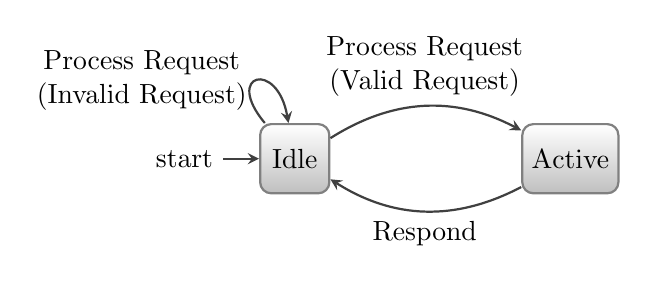
\begin{tikzpicture}[->,>=stealth', node distance=3.5 cm, thick]
    \tikzstyle{every state}=[rectangle,
                       draw=gray,
                       rounded corners,
                       rectangle,
                       top color=white,
                       bottom color=gray!50]
    \tikzstyle{every path}=[->,gray!150,>=stealth,text=black]
    \node[state, initial] (A) []      {Idle};
    \node[state]      (B) [right of=A]{Active};

    \path (A) edge[loop above,left, align=center, out=130,in=100, looseness=7]node{Process Request\\(Invalid Request)}(A)
          edge[bend left, above,  align=center]               node{Process Request\\(Valid Request)}  (B)
        (B) edge[bend left, below]                        node{Respond}             (A);
  \end{tikzpicture}
  \caption{FSM, describing the \ttt{Service} entity in Figure~\ref{fig:modelExProtocol}.}
  \label{fig:fsmExService}
\end{figure}

\section{Uses of model-based testing of the MCP}
The main advantage that comes from model-based testing is the large variety in testing algorithms it produces. If a model is to be machine readable the techniques, listed below can be implemented fully automatic, and if not, they can still be utilized manually. The following techniques can be applied to true and fair maritime service-models in the MCP: \newpage
\begin{description}
  \item[Finite state machines]\ \\
    As mentioned in Section~\ref{ssec:Finite State Machines (FSM)}, a FSM is made up of states, and the ability of a simulating program to change state through a collection of actions. Executable paths are determined, which can be used to create test cases, as well as illustrate the behavior of the system. Furthermore FSMs are closely related to the further techniques, that will be explained below.
  \item[Proving theorems]\ \\
    Automatic theorem proving is a technique originally produced for proving logical formulas, which is a concept that can be rewritten to suit model-based testing. In order to create test cases, system behavior is assigned to equivalence classes. Following this step, predicates can be formed from equivalence classes and logical consequences of the equivalence classes. 
  \item[Symbolic execution]\ \\
    Much in the likes of an FSM, a symbolic execution of a program or system will generate executable paths, along with symbolic values, describing how they can be accessed. A symbolic execution engine will analyze possible variations of input in order to create a map of the software in question. Said map can subsequently be used to better understand, test, and develop the software in question.
  \item[Model checkers]\ \\
    Model checkers, also known as property checkers, are methods of determining if an FSM meets a specific set of requirements. The model checkers detect if requirements are met, either by determining examples or counterexamples. When a path, representing either an example or a counterexample is discovered it is logged as a \tit{witness}, which can be mutated upon when generating test cases.
  \item[Markov chains]\ \\
    Markov chains are named after the Russian mathematician Andrew Markov, and are also known as usage models. A Markov chain, or usage model, is made up of two primary components; firstly an FSM, which represents every available action of a given system, and secondly an operational profile, which is a statistical indicator of what has been or will be used. The FSM is used by the operational profile in order to generate the statistical analysis, and the operational profile is used by the FSM to derive operational tests.
\end{description}
The scope of which features the above techniques will be able to test, will be deemed by the actual maritime service model, however, the expansive array of methods will cover maritime services extensively.
\section{Use-Cases}
In this section, I will present the utilization of the desired tool, that is implemented throughout Chapter~\ref{chp:Work/Design} using techniques described in Chapter~\ref{chp:Analysis}. This entails three examples, described in Figures~\ref{fig:useCaseVerifyFirst} through~\ref{fig:useCaseIncorrect}, and visualized in Figure~\ref{fig:useCaseDiagram}. Figures~\ref{fig:useCaseVerifyFirst} and~\ref{fig:useCaseVerifySecond} describe intended use of the implementation, while Figure~\ref{fig:useCaseIncorrect} describes unintended use of the implementation. Actor/system-interaction is described in Figure~\ref{fig:useCaseDiagram}.
\begin{figure}[h]
  \centering
  \begin{tabular}{l|l} \toprule
    Use Case   & System verifies model, first iteration \\ \midrule
    Actors     & Service Instance designer (SD) \\ \midrule
    Basic Flow & \makecell[l]{1. SD will submit a service specification.\\
                              2. SD submits all information as per the old service\\
                              \ \ \ \ specification syntax.\\
                              3. SD submits all information to generate maritime model. \\
                              4. Model concept is tested and accepted. \\
                              5. SD submits the service instance specification.}  \\ \bottomrule
  \end{tabular}
  \caption{First example of correct use of the solution.}
  \label{fig:useCaseVerifyFirst}
\end{figure}
\begin{figure}[h]
  \centering
  \begin{tabular}{l|l} \toprule
    Use Case   & System verifies model, second iteration \\ \midrule
    Actors     & Service Instance designer (SD) \\ \midrule
    Basic Flow & \makecell[l]{1. SD designer will submit a service specification.\\
                              2. SD submits all information as per the old service\\
                              \ \ \ \ specification syntax.\\
                              3. SD submits all information to generate maritime model. \\
                              4. Model concept is tested and rejected.\\
                              5. SD repeats step 3.\\
                              6. Model concept is tested and verified. \\
                              7. SD submits the service instance specification.}  \\ \bottomrule
  \end{tabular}
  \caption{Second example of correct use of the solution.}
  \label{fig:useCaseVerifySecond}
\end{figure}
The steps described in Figures~\ref{fig:useCaseVerifyFirst} and~\ref{fig:useCaseVerifySecond} are similar up until 4, where one example accepts, while the other example rejects the model. As the Service Instance Designer produces a valid model in Figure~\ref{fig:useCaseVerifyFirst}, the fact that the system is used correctly is trivial, and while the initial model is rejected, based on the desired behavior in Figure~\ref{fig:useCaseVerifySecond}, the final result is a valid model concept, and thus the software has been used as intended.
\newpage
\noindent
In the case of Figure~\ref{fig:useCaseIncorrect} a model is created, using the system, similar to above, however, the result of the checked input is ignored by the user. This should still be possible, as the limitations of the system, should not be projected onto the created software, but in some instances, it could also lead to invalid model-concepts being iterated upon further.
\begin{figure}[h]
  \centering
  \begin{tabular}{l|l} \toprule
    Use Case   & User ignores model warnings \\ \midrule
    Actors     & Service Instance designer (SD) \\ \midrule
    Basic Flow & \makecell[l]{1. SD designer will submit a service specification.\\
                              2. SD submits all information as per the old service\\
                              \ \ \ \ specification syntax.\\
                              3. SD submits all information to generate maritime model. \\
                              4. Model concept is tested and rejected.\\
                              5. SD submits the service instance specification.}  \\ \bottomrule
  \end{tabular}
  \caption{Incorrect use of the solution.}
  \label{fig:useCaseIncorrect}
\end{figure}
\begin{figure}
  \centering
  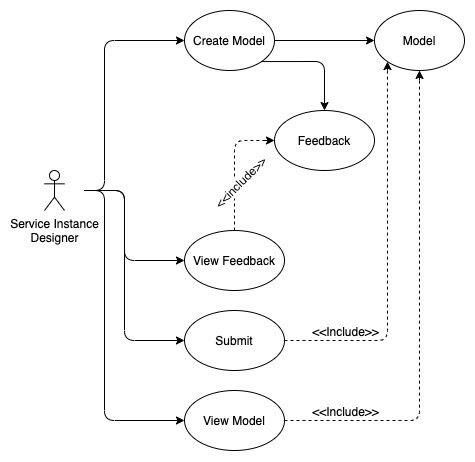
\includegraphics[width=0.8\linewidth]{figures/UCD.jpg}
  \caption{Use case diagram describing Figures~\ref{fig:useCaseVerifyFirst},~\ref{fig:useCaseVerifySecond}, and~\ref{fig:useCaseIncorrect}.}
  \label{fig:useCaseDiagram}
\end{figure}
\newpage
\section{Summary: Advantages and Disadvantages} 
Issues will inevitably present themselves with a project such as this, however the scope and nature of these issues will vary with each approach possible. As different approaches offer tailored advantages to circumvent correlating unique concerns, another set of unique concerns will necessarily present themselves. In this section I will sum up the approaches presented throughout Chapter~\ref{chp:Analysis}, along with their corresponding arising advantages and disadvantages.
\subsection{Manual model-creation}
\tbf{Advantages}
\begin{itemize}
  \item Manual model creation will have a shorter initial implementation time, as an arbitrary single model is faster to build than its auto-model-generator counterpart. 
  \item Built maritime service models can be fully customized at once in order to describe all aspects of its maritime service counterparts.
  \item Having customized each maritime service model to its corresponding maritime service counterpart allows for an equally customized test suite. Following this, the techniques, described in Section~\ref{sec:Uses of model-based testing of the MCP}, will allow for exhaustive tests via manual model-creating.
\end{itemize}
\tbf{Disadvantages}
\begin{itemize}
  \item The time consumption of manually creating each model will expand near-linearly with each maritime service, that is submitted, and subsequently needs a maritime service model. 
  \item Having each maritime service model being created individually and manually will inevitably introduce much diversity both in the sense of the available standard actions and implementation style of the model.
  \item The complexity as well as way of implementing testing techniques explained in Section~\ref{sec:Uses of model-based testing of the MCP} varies to an extent, even without consideration of non-uniform models. Elaborating on the case that each maritime service model differs both in purpose, implementation style and exhaustiveness, creating test suites similar to those described in Section~\ref{sec:Uses of model-based testing of the MCP} for each new maritime service, will become an extensive project.
\end{itemize}\newpage
\subsection{Automatic model-creation}
\tbf{Advantages}
\begin{itemize}
  \item The first and foremost advantage of automatic model generation is the scalability it provides. This comes as the implementation of \tit{one} maritime service model generator module, ideally, will be able to automatically assemble each maritime model without further interference, as opposed to manual model generating.
  \item As an automatic model generator abides by a set collection of rules and metrics, and would create models following the instructions of an xml specification-file, generated models will never deviate from the uniformity of the generator.
  \item The uniformity in the generated models will further show advantage, as this will streamline test suite generation either because of the fact that similar models promote similar manual test suite generation, or because that it allows for near-total automation.
\end{itemize}
\tbf{Disadvantages}
\begin{itemize}
  \item The obvious disadvantage that comes with automatic model generation, is the lack of customization in models. As the generator should handle all models that can be described through the xml specification files, it needs to be generalized, which in turn means less specific models, which lowers the ability to custom-fit each model to its maritime specification counterpart.
  \item Another inevitable downside of having automatically generated - however less specific - models is the fact that test suites can become less specific, and in extension hereof less exhaustive of the maritime service.
\end{itemize}
\indent
To sum up, both methods will be advantageous, as they will each allow for extensive testing, with the former being more custom-tailored and so a lot more time consuming in the long run, and the latter being more generic, but much ultimately less time consuming in the long run.
\displayCounterChp
%%%%%%%%%%%%%%%%%%%%%%%%%%%%%%%%%%%%%%%%%%%%%%%%%%%%%%%%%%%%%%%%%%%%%%%%%%%%%%%
%%% Work                                                                    %%%
%%%%%%%%%%%%%%%%%%%%%%%%%%%%%%%%%%%%%%%%%%%%%%%%%%%%%%%%%%%%%%%%%%%%%%%%%%%%%%%

\chapter{Work/Design}

In this chapter I will describe the work I have done in order to implement model-based testing into the MCP. The workload that is contained in the implementation and description herein includes implementation of a monadic parser that reads the xml-specification files, an update of the fields and contents of fields in the xml-specification files, as well as a model, that is built upon the foundation of aforementioned updated xml-specification.
\TODOOPT{Hvis det fungerer med interpreter(parser(xml))=model, så skriv det på.}
\section{Updated Data}

As discussed in Section \ref{sec:Data}, in order to create uniform models, upon which to execute tests, the structure of the xml-specification files needs to be altered in a manner that adds uniformity to the xml-specification files. This rules out the use of natural language, for reliable model-generation.

One way to implement these changes is make the user able to assign variables, based on a fixed collection of available options. I will now present three fields, which are designed to be used in order to maximize uniformity in model generation as well as give maximum flexibility in future model design.

\TODO{Does not fitt 100 \% with the implemented}
\begin{description}
	\item[Entity]\ \\
	An entity is the most basic component of the models, without which, the models would not be able to exist. These describe the physical real-world objects, which the model is to simulate, and these are also the subjects of all transactions, which will occur throughout execution of the models. At the moment, three entities exist, however support for additional models is possible.
	\begin{description}
		\item[Ship]\ \\
		If comparing the MCP to the App Store or Google Play, a ship would undertake the role of the user. The user can be the one utilizing the maritime service or in other cases other users, which are somehow connected to the user. 
		\item[Service]\ \\
		The Service entity represents the maritime service, which is being modeled. Like a ship entity, multiple instances of a service entity can occur. If multiple instances of a service entity occurs, this will correspond to cross app interaction, using the same comparison as above.
		\item[Company]\ \\
		Company entities serve as nodes, which hold data or other goods, which can be desired by ship entities for a variety of reasons. Multiple company entities can exist at one time. 
	\end{description}
	\item[Relation]\ \\
	A relation symbolizes a bond between two entities. In the case of Figure \ref{fig:modelExProtocol}, relations can be seen between 'Ship' and 'Service' as well as 'Service' and 'Company'.

	A ship entity can share a relation with other ship entities, as well as service entities, but in order to access data held by the company entity, it will need to consult the service entity.

	A service entity needs to be able to share a relation with all other entities in order to act as an intermedium between ship entities and company entities, while also being able to interact with other service entities.

	A company entity can share a relation with a service entity as well as other company entities. Two company entities do not necessarily need service entities in order to be able to share information similarly to the real world, where companies use different communication channels, whether communicating with companies or citizens.
	\item[Dependency]\ \\
	A dependency is, as the name suggests, a dependency from one entity to another, and so the first argument of a dependency must be a relation, which describes which two entities are in question, as well as which entity depends on the other. The second argument that a dependency must receive is an anonymous function, that describes what the entities require from each other. If two entities co-depend on each other a relation must be made from the first to the second, as well as from the second to the first. As only the anonymous function limits what the dependency entails, an entity \tit{can} depend on itself.
\end{description}

Figure \ref{fig:entities} describe which options are excluded at selections of entities, relations, and dependencies. As can be seen, Figure \ref{fig:entities} coincides with \ref{fig:sSpecUpd}, and therefor the description given in this section describe both figures. 

\begin{figure}
	\centering
	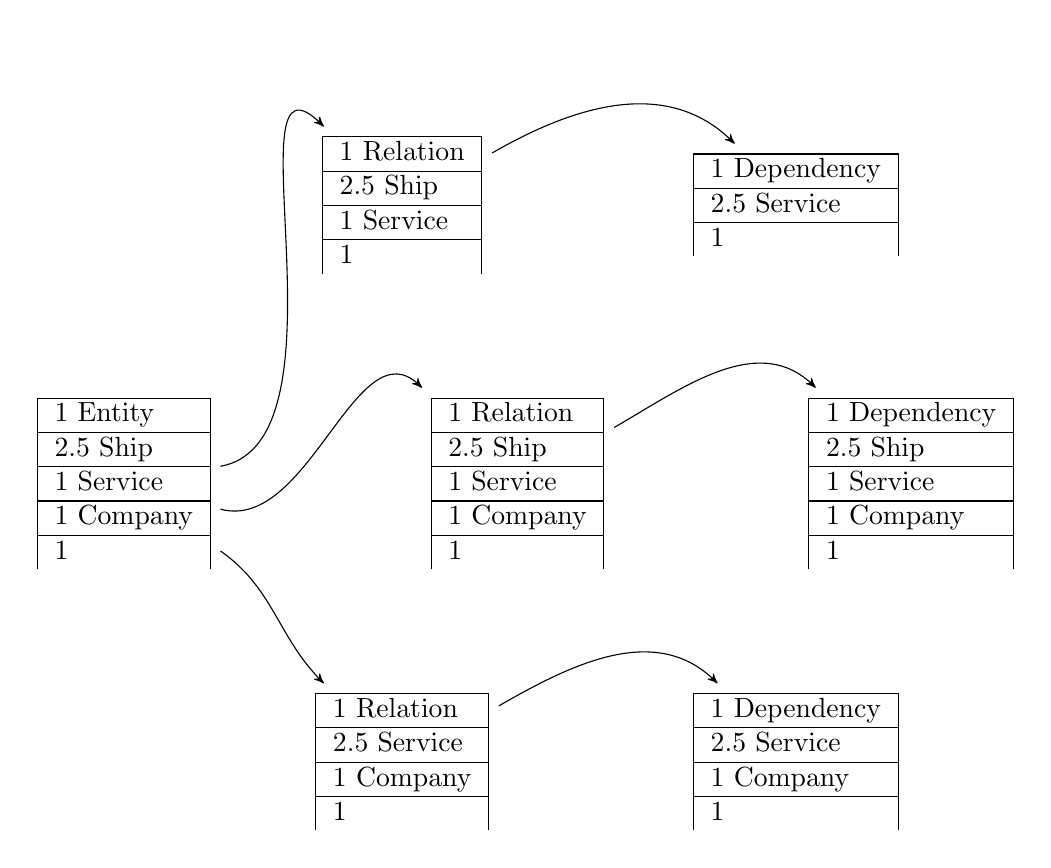
\begin{tikzpicture}[->,>=stealth', node distance=5 cm]
		\node[]	(A)	[]	
			{\begin{tabular}{|l|}\hline{1}
				Entity         \\ \hline{2.5}
				Ship            \\ \hline{1}
				Service          \\ \hline{1}
				Company	          \\ \hline{1}
			\end{tabular}};
		\node[]	(B)	[above right of=A]
			{\begin{tabular}{|l|}\hline{1}
				Relation       \\ \hline{2.5}
				Ship            \\ \hline{1}
				Service          \\ \hline{1}
			\end{tabular}};
		\node[]	(C)	[right of=A]
			{\begin{tabular}{|l|}\hline{1}
				Relation       \\ \hline{2.5}
				Ship            \\ \hline{1}
				Service          \\ \hline{1}
				Company           \\ \hline{1}
			\end{tabular}};
		\node[]	(D)	[below right of=A]
			{\begin{tabular}{|l|}\hline{1}
				Relation       \\ \hline{2.5}
				Service         \\ \hline{1}
				Company          \\ \hline{1}
			\end{tabular}};
		\node[]	(E)	[right of=B]
			{\begin{tabular}{|l|}\hline{1}
				Dependency     \\ \hline{2.5}
				Service          \\ \hline{1}
			\end{tabular}};
		\node[]	(F)	[right of=C]
			{\begin{tabular}{|l|}\hline{1}
				Dependency     \\ \hline{2.5}
				Ship            \\ \hline{1}
				Service          \\ \hline{1}
				Company           \\ \hline{1}
			\end{tabular}};
		\node[]	(G)	[right of=D]
			{\begin{tabular}{|l|}\hline{1}
				Dependency     \\ \hline{2.5}
				Service         \\ \hline{1}
				Company          \\ \hline{1}
			\end{tabular}};
		\path	(A)	edge	[out=10]	node	{}	(B)
					edge	[out=345]	node	{}	(C)
					edge	[out=325]	node	{}	(D)
				(B)	edge	[out=30]	node	{}	(E)
				(C)	edge	[out=30]	node	{}	(F)
				(D)	edge	[out=30]	node	{}	(G);
	\end{tikzpicture}
	\caption{Available relations and dependencies for ships, services, and companies}
	\label{fig:entities}
\end{figure}


\section{Updated Parser Grammars}

The fields described in Section \ref{sec:Updated Data} furthermore need to be translated into parsable xml, and an example of this is given in Listing \ref{fig:sSpecUpd}. This parser grammar serves as an updated version of the parser grammar, described in Listing \ref{fig:sSpecFull}, however shaved for information\footnote{aSpec, authorInfo, authorInfos, contactInfo, dataExchangePattern, definitionAsXSD, description, isSpatialExclusive, keywords, oSpec, operation, operations, parameterType, parameterTypes, ptSpec, rSpec, requirement, requirements, returnValueType, serviceDataModel, serviceInterface, serviceInterfaces, siSpec, spec, specifications, status, text, typeReference, version}, that is irrelevant to the model-generating process. While this information can of course be included in the xml-specification file, it will be deemed irrelevant after parsing, and thus not included further in the model-generating process. The parser grammar presented in Listing \ref{fig:sSpecUpd} is designed to form a clear and unambiguous collection of entities, along with a similarly unambiguous description of relations, exchange-patterns, and security precautions. The parser grammar abides by the rules, presented in Section \ref{sec:Updated Data} and Figure \ref{fig:entities}.

\subsection{Updated Service Specification Grammar}

\begin{figure}
	\centering
	\begin{lstlisting}[keywordstyle={}]
ServiceSpecificationSchema ::= specifications

specifications ::= spec specifications
     | $\e$
     
spec ::= name
     | status
     | id
     | Entities

Entities ::= ESpec Entities
     | $\e$

ESpec ::= Ship
     | Service
     | Company

Ship ::= name
     | id
     | Relations

Service ::= name
     | id
     | Relations
     | Dependencies

Company ::= name
     | id
     | Relations

Relations ::= RSpec Relations
     | $\e$

RSpec ::= ESpec ESpec

Dependencies ::= DSpec Dependencies
     | $\e$

DSpec ::= Dependency RSpec
	\end{lstlisting}
	\caption{Updated parser grammar of Service Specification Schema}
	\label{fig:sSpecUpd}
\end{figure}
\subsection{Updated General Grammar}
The updated xml-specification files will be limiting the flexibility of the models in some aspects, as not all maritime services would follow the structure given in Listing \ref{fig:sSpecUpd}, however the example given is the earliest version of the domain-specific language. Following complex structures of various maritime services, the domain-specific language of the specification files can scale in complexity with the requirements set up by the maritime services.

Listing \ref{fig:sSpecUpdRed} describes a reduced form of Listing \ref{fig:sSpecUpd}. It can be seen that Listing \ref{fig:sSpecUpdRed} is identical to Listing \ref{fig:sSpecRed}, which proves that, after implementation of the model-generating process, there is no direct, urgent need to improve or change the parser.

\begin{figure}
	\centering
	\begin{lstlisting}[keywordstyle={}]
ServiceSpecificationSchema ::= specifications

specifications ::= spec specifications
     | $\e$
     
spec ::= specifications
     | spec
     | $\e$

spec ::= string
	\end{lstlisting}
	\caption{Reduced parser grammar of the updated Service Specification Schema}
	\label{fig:sSpecUpdRed}
\end{figure}

\section{Implementation in the MCP}
\TODO{Hvordan skal dette implementeres/BRUGES i MCP (ikke teknisk)}

\section{Technical Implementation}
\TODO{Evt lav nedenstående til et Chapter}

\subsection{Executing Instructions}
\TODO{ }

\section{Testing}
\TODO{ }


\displayCounterChp

%%%%%%%%%%%%%%%%%%%%%%%%%%%%%%%%%%%%%%%%%%%%%%%%%%%%%%%%%%%%%%%%%%%%%%%%%%%%%%%
%%% Experiments and Results                                                 %%%
%%%%%%%%%%%%%%%%%%%%%%%%%%%%%%%%%%%%%%%%%%%%%%%%%%%%%%%%%%%%%%%%%%%%%%%%%%%%%%%

\chapter{Experiments and Results}

\begin{figure}
	\centering
	\begin{lstlisting}[keywordstyle={}]
Term =
    {entities,
        [{ent,
             [{type,"ship"},
              {name,"Ship"},
              {relations,[{relation,"Service"}]},
              {dependencies,
                  [{dependency,[{to,"Service"},{constraint,"fun psswd"}]},
                   {dependency,[{to,"Service"},{constraint,"fun user"}]}]},
              {information,[]},
              {requests,
                  [{request,
                       [{to,"Service"},
                        {data,"map"},
                        {answers,[{answer,"anton"},{answer,"1234"}]}]}]}]},
         {ent,
             [{type,"service"},
              {name,"Service"},
              {relations,[{relation,"Ship"},{relation,"Company"}]},
              {dependencies,[]},
              {information,[]},
              {requests,[]}]},
         {ent,
             [{type,"company"},
              {name,"Company"},
              {relations,[{relation,"Service"}]},
              {dependencies,[]},
              {information,[{info,"map"}]},
              {requests,[]}]}]}
	\end{lstlisting}
	\caption{Erlang term, resulting of parsing the file \ttt{protocol.xml} with \ttt{main:parse('xml/protocol.xml')}}
	\label{fig:protocolParsed}
\end{figure}


\begin{figure}
	\centering
	\begin{lstlisting}[keywordstyle={}]
[{company,[{<0.96.0>,[]}],<0.95.0>,["map"]},
 {service,[{<0.95.0>,[]},{<0.97.0>,[]}],<0.96.0>,[]},
 {ship,[{<0.96.0>,
         [#Fun<aux.1.64654801>,#Fun<aux.0.64654801>]}],
       <0.97.0>,
       ["map"]}]
	\end{lstlisting}
	\caption{Maritime model, resulting of interpreting the file \ttt{protocol.xml} with \ttt{main:parse\_and\_interpret('xml/protocol.xml')}}
	\label{fig:protocolParsedInterpreted}
\end{figure}

\begin{figure}
  \centering
  \begin{lstlisting}[keywordstyle={}]
[{company,[{<0.79.0>,[]}],<0.80.0>,["map"]},
 {service,[{<0.78.0>,[]},{<0.80.0>,[]}],<0.79.0>,[]},
 {ship,[{<0.79.0>,
         [fun aux:user/1,fun aux:psswd/1]}],
       <0.78.0>,
       ["map"]}]
  \end{lstlisting}
  \caption{Maritime model, resulting of executing the commands, contained within the function \ttt{examples:protocol}}
  \label{fig:protocolManual}
\end{figure}

\displayCounterChp

%%%%%%%%%%%%%%%%%%%%%%%%%%%%%%%%%%%%%%%%%%%%%%%%%%%%%%%%%%%%%%%%%%%%%%%%%%%%%%%
%%% Discussion                                                              %%%
%%%%%%%%%%%%%%%%%%%%%%%%%%%%%%%%%%%%%%%%%%%%%%%%%%%%%%%%%%%%%%%%%%%%%%%%%%%%%%%

\chapter{Discussion}
Following the successful development of the solution, described in the preceding chapters, problem statements arise dealing with integration into the MCP, use, future use and the balancing of the compromise that is choosing which model generator to utilize. The following chapter will deal with these topics. Section ~\ref{sec:Launch and Integration into the MCP} will describe potential approaches to initial integration, while Section~\ref{sec:Future Use} will describe the subsequent future use, both practical and technical, following the inevitable need for further development. Section~\ref{sec:Manual versus Automatic Model Generation}, will contain an assessment of which model generating functionality is most likely to be widely used, going forward. Eventually, Section~\ref{sec:Results Related to Use} will provide a recap of the results obtained in Chapter~\ref{chp:Results}, in relation to what is described in sections~\ref{sec:Launch and Integration into the MCP} through~\ref{sec:Results Related to Use}.

\section{Launch and Integration into the MCP}
For the solution described throughout this thesis to be integrated, various changes need to be made with regards to the infrastructure of the Maritime Connectivity Platform. The first, and most obvious, change that should be implemented is the technical implementation of the new functionality. Next comes the need for educating the user-group, as these will have no preceding knowhow as to make the system work in accordance with their needs. This will be necessary whether use of manual or automatic model generating is utilized, however, can be largely solved b an extensive user guide.

A soft launch strategy should be used when inaugurating the functionality, as described in a blog-post on LiveChatInc~\cite{hardoSoft}. Launching the solution gradually will let the user-base get acquainted with its use, while simultaneously allowing for necessary feedback towards the functionality. This will, in turn, decrease the risk of the project succumbing to any of the launch failures, as described in an article on Harvard Business Review~\cite{hbr}, all of which are often connected with a hard product launch.
\section{Future Use}
Post-launch of the model-building component will be a continuous development process. User-submitted feedback should be regularly implemented in order to ensure optimal user friendliness, and intuitiveness. Furthermore, the functionality described in Chapter~\ref{chp:Work/Design} is only the initial functionality, and ideally, as described in Section~\ref{ssec:Expanding Automatic Model Functionality} below, future development is deeply rooted in the project.

\subsection{Expanding Automatic Model Functionality}
Embedded in the nature of the project is the need for future expansion of functionality, following increased demands from maritime service providers. The modularity that the solution has been implemented with will aid in this, as it allows for less complicated employment hereof. As described in Section~\ref{sec:Technical Implementation}, the complete solution has been divided into three fields, and thus, these are the areas where further implementation is needed, if support for additional model functionality is desired.
\begin{itemize}
  \item \ttt{mmods.erl}\\
    The primary functionality will need to be implemented here. This entails the main API call to the finite state machine, along with its following desired result and side effects. Altering the implementation of this file will subsequently alter the manual as well as the automatic model generator.
  \item \ttt{parser.erl}\\
    This file will \tit{not} need any adjustments in order to handle new functionality.
  \item \ttt{interpreter.erl}\\
    This file will need to be altered in order to handle additional information, picked up by the parser. In the case that support for model functionality has been implemented in \ttt{mmods.erl}, but not \ttt{interpreter.erl}, said functionality will not be included in the resulting model, and no error or exception will be raised. This is true, even if the additional design information is included in the xml specification file that is parsed and interpreted.
\end{itemize}

\subsection{Expanding Manual Model Functionality}
As explained in Section~\ref{ssec:The parser and interpreter modules}, the manual component provides all core functionality of the automatic component. The fact that this module is underdeveloped in comparison to its automatic counterpart, in no way rules out its future use, as having only the core functionality encapsulated in a module, providing an all-inclusive API allows for virtually limitless further development. The automatic component is \tit{one} example out of a virtually endless pool of additional, untapped functionality, based on the functionality, provided in the manual component. Expanding upon this will be confined to future work, as potential solutions can scope to an extent similar to this project.

\section{Manual versus Automatic Model Generation}
A fundamental obstacle throughout the project is the learning curves, described in Figures~\ref{fig:serialMBT} and~\ref{fig:sequenceMBT}, along with their corresponding sections. This obstacle is present in both scenarios, however, the learning curve is significantly steeper, using sequential\footnote{Manual} model based testing/model generating. A soft launch and extensive user-guide, as described in Section~\ref{sec:Launch and Integration into the MCP}, will reduce the effects of the learning curve for both development techniques, however, not to the extend that this is completely negated.

Automatic model generation is, however, both the most user-friendly method and the one most suited for a visual builder interface. A visual builder interface could be in a style, similar to the Eclipse Visual Editor, Vex~\cite{vex} for XML. Such an XML-builder should be implemented to always show the user which options are available to add to the xml and subsequent model, which would in turn ease work flow, placed on all other aspects of the solution.

\section{Results Related to Use}
Taking the findings of Chapter~\ref{chp:Results} into consideration, when comparing the usefulness of the two methods, one model-generating technique clearly stands out as being the most useful. That is, automatic model-generation will provide more immediate user-friendliness, more scalability, and according to Section~\ref{ssec:Model Equivalence}, functionality equivalent to that of manual model-generation.

A central perk of the solution is to, through model-based testing, visualize and predict intended behavior of maritime services. Being able to do this, will not only be advantageous in the ability to create software, more in the likes of what is desired; it will also speed up the process of doing so. Most development processes are implemented, using the much praised Scrum~\cite{scrum} framework. Developing software, using the Scrum framework entails a circular approach to the way the process plays out. Typically, such a process starts with the basic idea of the application. After this step, a loop starts with planning and analysis of intended functionality and behavior, followed by implementation, functionality and behavioral testing, and lastly, revision. After revision, the process initiates once again, beginning with planning and analysis.
\newpage
\noindent
Figure~\ref{fig:scrumBig} visualizes a standard scrum framework, which can be followed, when developing a maritime service. The scrum method in question, although agile, can be a lengthy process, partly because of the `testing' sequences. Furthermore `Implementation' and `Revision' may, in the worst cases, be performed to little benefit, if performed on the basis of a faulty design.
\begin{figure}[h]
  \centering
  \smartdiagramset{
    set color list={gray!50,gray!50,gray!50,gray!50,gray!50},
    arrow line width=2 pt
  }
    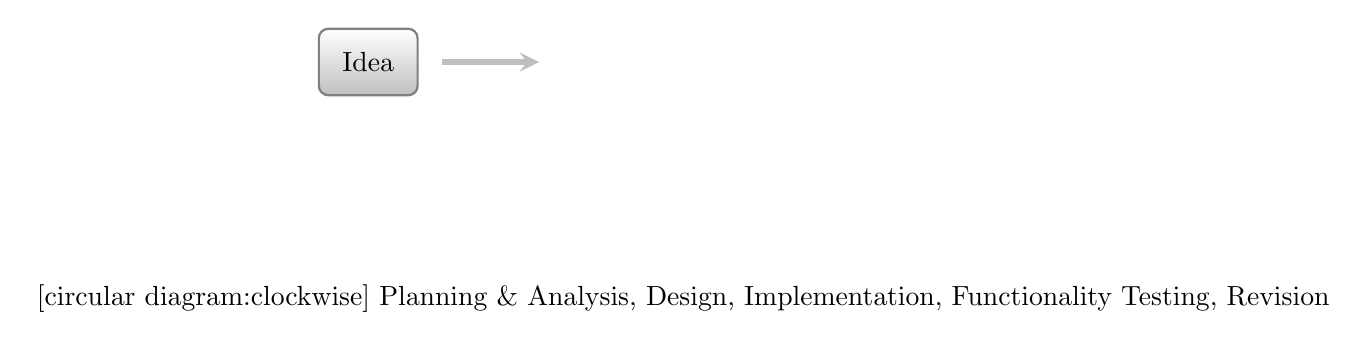
\begin{tikzpicture}[thick]
    \node at (0,0)   {\smartdiagram[circular diagram:clockwise]{
      Planning \& Analysis,
      Design,
      Implementation,
      Functionality Testing,
      Revision}
    };

    \node [rectangle,
           draw=gray,
           rounded corners=0.12 cm,
           inner sep=0.3 cm,
           top color=white,
           bottom color=gray!50]
          (S)  at (-4,3)  {Idea};

    \node (DevI) at (-1.7,3) {};
    \node (StaO) at (-3.2,3) {};

    \path [->,line width=2 pt,gray!50,>=stealth] (StaO) edge (DevI);
  \end{tikzpicture}
  \caption{Scrum development cycle without automated model-based testing.}
  \label{fig:scrumBig}
\end{figure}

The automatic model-generator, described in Section~\ref{sec:Technical Implementation}, can aid in the issue, defined above. The tool will allow users to visualize an intended version of their maritime service instance, before initializing implementation, which will enable them to skip the steps `Implementation', `Functionality Testing', `Revision', and `Planning \& Analysis' in a given scrum cycle. In an ideal use case scenario, such as the one, described in Figure~\ref{fig:useCaseVerifySecond}, as crucial information is given before advancement, a user can, thus, skip large portions of cycles, thereby saving time by not follow dead design ends.

This principle is described by Figure~\ref{fig:scrumSmall}, where `Behavioral Testing' is added to a sub-cycle, only shared with `Design', thereby creating a much smaller, and considerably faster, sprint.
\newpage
\begin{figure}[h]
  \centering
  \smartdiagramset{arrow line width=2 pt}
  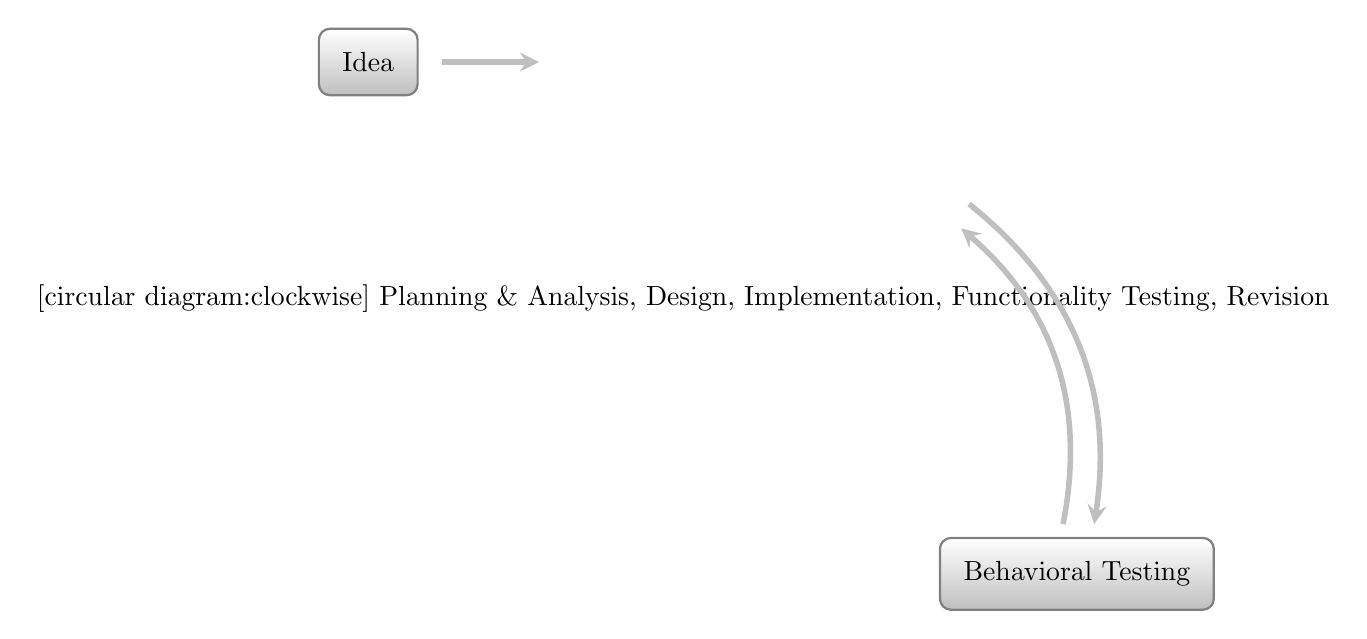
\begin{tikzpicture}[thick]
    \node at (0,0) {\smartdiagram[circular diagram:clockwise]{
      Planning \& Analysis,
      Design,
      Implementation,
      Functionality Testing,
      Revision}
    };

    \node [rectangle,
           draw=gray,
           rounded corners,
           inner sep=0.3 cm,
           top color=white,
           bottom color=gray!50]
          (S)  at (-4,3)  {Idea};

    \node [rectangle,
           draw=gray,
           rounded corners,
           inner sep=0.3 cm,
           top color=white,
           bottom color=gray!50]
          (FT)  at (5,-3.5)  {Behavioral Testing};

    \node (DevI) at (-1.7,3) {};
    \node (StaO) at (-3.2,3) {};

    \node (DI)  at (3.5,1.3) {};
    \node (DO)  at (3.4,1) {};

    \node (FTI) at (4.8,-3) {};
    \node (FTO) at (5.2,-3) {};

    \path [->,line width=2 pt,gray!50,>=stealth] (StaO) edge (DevI) 
          [bend left]                            (DI)   edge (FTO)
          [bend right]                           (FTI)  edge (DO);
  \end{tikzpicture}
  \caption{Scrum development cycle with automated model-based testing.}
  \label{fig:scrumSmall}
\end{figure}

Manual model generation, in it's basic state, as described in Section~\ref{ssec:Expanding Manual Model Functionality}, allows for limitless new functionality, and, as proven by the implementation of the automatic component, said new functionality does not necessarily need to be manual.\\[0.5cm]
In conclusion, both components add relevant functionality to the MCP, and while automatic model generating provides the more present, needed, utility, the manual component provides a broad foundation for development of new ideas.


\displayCounterChp

%%%%%%%%%%%%%%%%%%%%%%%%%%%%%%%%%%%%%%%%%%%%%%%%%%%%%%%%%%%%%%%%%%%%%%%%%%%%%%%
%%% Conclusion                                                              %%%
%%%%%%%%%%%%%%%%%%%%%%%%%%%%%%%%%%%%%%%%%%%%%%%%%%%%%%%%%%%%%%%%%%%%%%%%%%%%%%%

\chapter{Conclusion}
In this chapter, I will conclude the results of my analysis and work. This includes a breakdown of what has been achieved the model-generating implementation, as well as suggestions to what can be achieved, by expanding upon the project in future work in Section \ref{sec:Future Work}. Section \ref{sec:Summary} contains a summary, describing key takeaways from the thesis in bullet-point form.
\section{Conclusions}
In Chapter \ref{chp:Background}, an assessment was provided of methods, which could be utilized to implement a solution to the problem that was also described in Chapter \ref{chp:Introduction}. Specifically, the methods, that were utilized in the solution were the combination of a parser and an interpreter, which would feed commands to a finite state machine, thereby creating the maritime models. This process of implementing this was described in Chapter \ref{chp:Work/Design}, and the process of determining this design is described in Chapter \ref{chp:Analysis}.

In Chapter \ref{chp:Results}, I verified the validity of the operations, performed in the implementation through extensive testing. That is, the testing, performed in Section \ref{sec:Testing}, concluded that the model creators, described throughout Chapter \ref{chp:Work/Design} could create working models, which adhered to the set of rules and descriptions, described in Chapter \ref{chp:Analysis}. 
\section{Future Work}

\subsection{Expandability}
%lazy evaluation
%modularity
%Monadic parser
\subsection{Automated Testing}
%Model-testing opposed to example-testing (Create a model, identify test-entities, do teststuff)

\section{Summary}

\displayCounterChp

%%%%%%%%%%%%%%%%%%%%%%%%%%%%%%%%%%%%%%%%%%%%%%%%%%%%%%%%%%%%%%%%%%%%%%%%%%%%%%%
%%% BIBLIOGRAPHY                                                            %%%
%%%%%%%%%%%%%%%%%%%%%%%%%%%%%%%%%%%%%%%%%%%%%%%%%%%%%%%%%%%%%%%%%%%%%%%%%%%%%%%

\cleardoublepage
\renewcommand{\sc}[1]{\textsc{#1}}
\bibliographystyle{acm}
\bibliography{bibliography}

%%%%%%%%%%%%%%%%%%%%%%%%%%%%%%%%%%%%%%%%%%%%%%%%%%%%%%%%%%%%%%%%%%%%%%%%%%%%%%%
%%% RESEARCH PAPERS                                                         %%%
%%%%%%%%%%%%%%%%%%%%%%%%%%%%%%%%%%%%%%%%%%%%%%%%%%%%%%%%%%%%%%%%%%%%%%%%%%%%%%%

\begin{thebibliography}{9}
	\bibitem{mcp}
		Maritime Connectivity Platform,
		\url{https://maritimeconnectivity.net/}
	\bibitem{quickcheck}
		QuickCheck,
		\url{http://hackage.haskell.org/package/QuickCheck}
	\bibitem{efficienSea2}
		EfficienSea2's website,
		\url{https://efficiensea2.org/solution/maritime-connectivity-platform/}
	\bibitem{realWorldHaskell11}
		Real World Haskell,
		Bryan O'Sullivan, Don Stewart, and John Goerzen,
		Chapter 11,
		\url{http://book.realworldhaskell.org/read/testing-and-quality-assurance.html}
	\bibitem{nlp}
		Natural Language Processing,
		Elizabeth D. Liddy,
		Syracuse University,
		\url{liddy@syr.edu}
		\url{http://surface.syr.edu/cgi/viewcontent.cgi?article=1019&context=cnlp}
	\bibitem{memoization}
		Monadic Memoization towards Correctness-Preserving Reduction of Search
		Richard Frost
		School of Computer Science, University of Windsor
		Ontario, Canada
		\url{richard@uwindsor.ca}
		\url{http://richard.myweb.cs.uwindsor.ca/PUBLICATIONS/AI_03.pdf}
	\bibitem{xmerl}
		xmerl reference manual,
		\url{http://erlang.org/documentation/doc-5.4/pdf/xmerl-1.0.pdf}
	\bibitem{xmerlEx}
		Starting to play with xmerl,
		Arif Ishaq,
		\url{https://arifishaq.wordpress.com/2014/11/25/starting-to-play-with-xmerl/}
\end{thebibliography}


\appendix

\chapter{Appendix}
\displayCounters
% Each paper is defined as a new section of an appendix chapter. This means that they automatically are added to TOC and it is possible to refer to them.

% Updates section names to remove . (e.g. a section is named A1 instead of A.1)
\renewcommand{\thesection}{\thechapter\arabic{section}}

\end{document}

% Til vejledning?
%
%	- Baggrund skal være længere (40/50 sider i alt er fino)
%		- beskriv teknikker (property/model-based testing)
%
%	- lav i første omgang en model på baggrund af min specifikation (manuel)
%	- lav i anden omgang en model på baggrund af min specifikation (automatisk)
